%\documentclass[a4j,10pt]{ujarticle}
\RequirePackage{ifuptex,ifluatex}
\ifluatex
\documentclass{ltjsarticle}
\else
\ifupTeX
\documentclass[uplatex,dvipdfmx]{ujarticle}
\else
\documentclass[dvipdfmx]{jarticle}
\fi
\fi
%\usepackage[dviout]{graphicx}
\usepackage{graphicx}
%%%%%%%%%%%%%%%%%%%%%%%%%%%%%%%%%%%%%%%%%%%%%%%%%%%%%%%%%%%%%%%%%%%%%

\pagestyle{empty}
\sloppy\fussy
\setlength{\topmargin}{-20.4mm}
\setlength{\textheight}{271mm}
\setlength{\textwidth}{175mm}
\setlength{\oddsidemargin}{-5.4mm}
\setlength{\evensidemargin}{-5.4mm}
\setlength{\headheight}{0mm}
\setlength{\footskip}{10mm}
\renewcommand{\baselinestretch}{0}
\renewcommand{\textfraction}{0}\renewcommand{\floatpagefraction}{1}
\renewcommand{\topfraction}{1} \renewcommand{\bottomfraction}{1}
%%%%%%%%%%%%%%%%%%%%%%%%%%%%%%%%%%%%%%%%%%%%%%%%%%%%%%%%%%%%%%%%%%%%%
\begin{document} 
\twocolumn[
\begin{center}
{\Large TCP並列接続を用いたプログレッシブダウンロード\\における順序制御方式の実装}\\
\vspace{1mm}
{\large Implementation of Sequence Control Method in Progressive Download \\
	Using Parallel TCP Connections}\\
\vspace{1mm}
{\large 1420180  平城 光雄 Mitsuo Heijo}\\
{\large 指導教員\ \  舟阪 淳一}\\
\end{center}
\vspace{-3mm}
]
\fontsize{9.6pt}{0pt}\selectfont
\section{はじめに}
\vspace{-3mm}
近年,効率的なコンテンツ配信を目的としたCDN等でのコンテンツの分散配置などが既に運用されている.
このような同一のファイルが分散配置されている状況を利用して複数のサーバと同時に通信を行うことで,より高速なファイルの取得を実現する方式が提案されている\cite{mhttp}\cite{proxy}.
しかし,既存の提案ではプログレッシブダウンロードにおける動画再生等を考慮した順序制御は目的とされていない.
本研究では,性能差のある複数のTCP接続を利用して異なるサーバから同一のファイルを分割取得する場合を想定し,要求送信時に各接続間の性能を比較することで到着順序逆転を抑制する順序制御方式を提案する.
\vspace{-8mm}

\section{関連研究}
\vspace{-3mm}
既存研究では,複数のサーバからファイルを分割して並列ダウンロードし,順序通りにクライアントに提供する代理サーバが提案されている\cite{proxy}.
既存の提案である重複再要求方式では,非有効ブロックの個数がある閾値を超えた場合は別の接続に要求を再送信することで事後的に順序逆転に対処していた.
この提案では,要求送信時における予防的な順序逆転への対策は行われていない.
また,動画等の再生を考慮した評価も行われていない.
\vspace{-8mm}

\section{提案方式}
\vspace{-3mm}
確立したTCP接続群の中で最高性能の接続には,最若番のブロックを要求する.
ここでの最高性能の定義は使用回数が最多の接続とする.
低性能の接続には前回の要求送信時からブロック到着までのブロック総受信回数の差分\begin{math}D\end{math}を計測し,
\begin{math}D\end{math}に基づいて最若番でないブロックを要求する.
\begin{math}D\end{math}は式\ref{eq}から求める.
\begin{math}T\end{math}はその時刻でのブロックの総受信回数,
\begin{math}P[X]\end{math}は接続\begin{math}X\end{math}の前回のブロック到着時におけるブロックの総受信回数,
\begin{math}N\end{math}は接続の個数である.
図\ref{delay}に2つの接続間に2倍の性能差がある場合の模式図を示す.
\begin{math}t=0\end{math}では遅延要求を行っていないので
\begin{math}t=1\end{math}にブロック1が到着しても,
ブロック0が到着していないのでブロック1は再生できない.
\begin{math}t=2\end{math}では
\begin{math}T=3, P[B]=0, N=2\end{math}であるので
接続Bに\begin{math}D=2\end{math}としてブロック要求を送信することで,
ブロック3-5が順序通りに到着している様子を示している.
\vspace{-3.5mm}
\begin{equation}
	\label{eq}
	D = T - P[X] - N + 1
\end{equation}
\vspace{-8mm}
\begin{figure}[h]
	\centering
	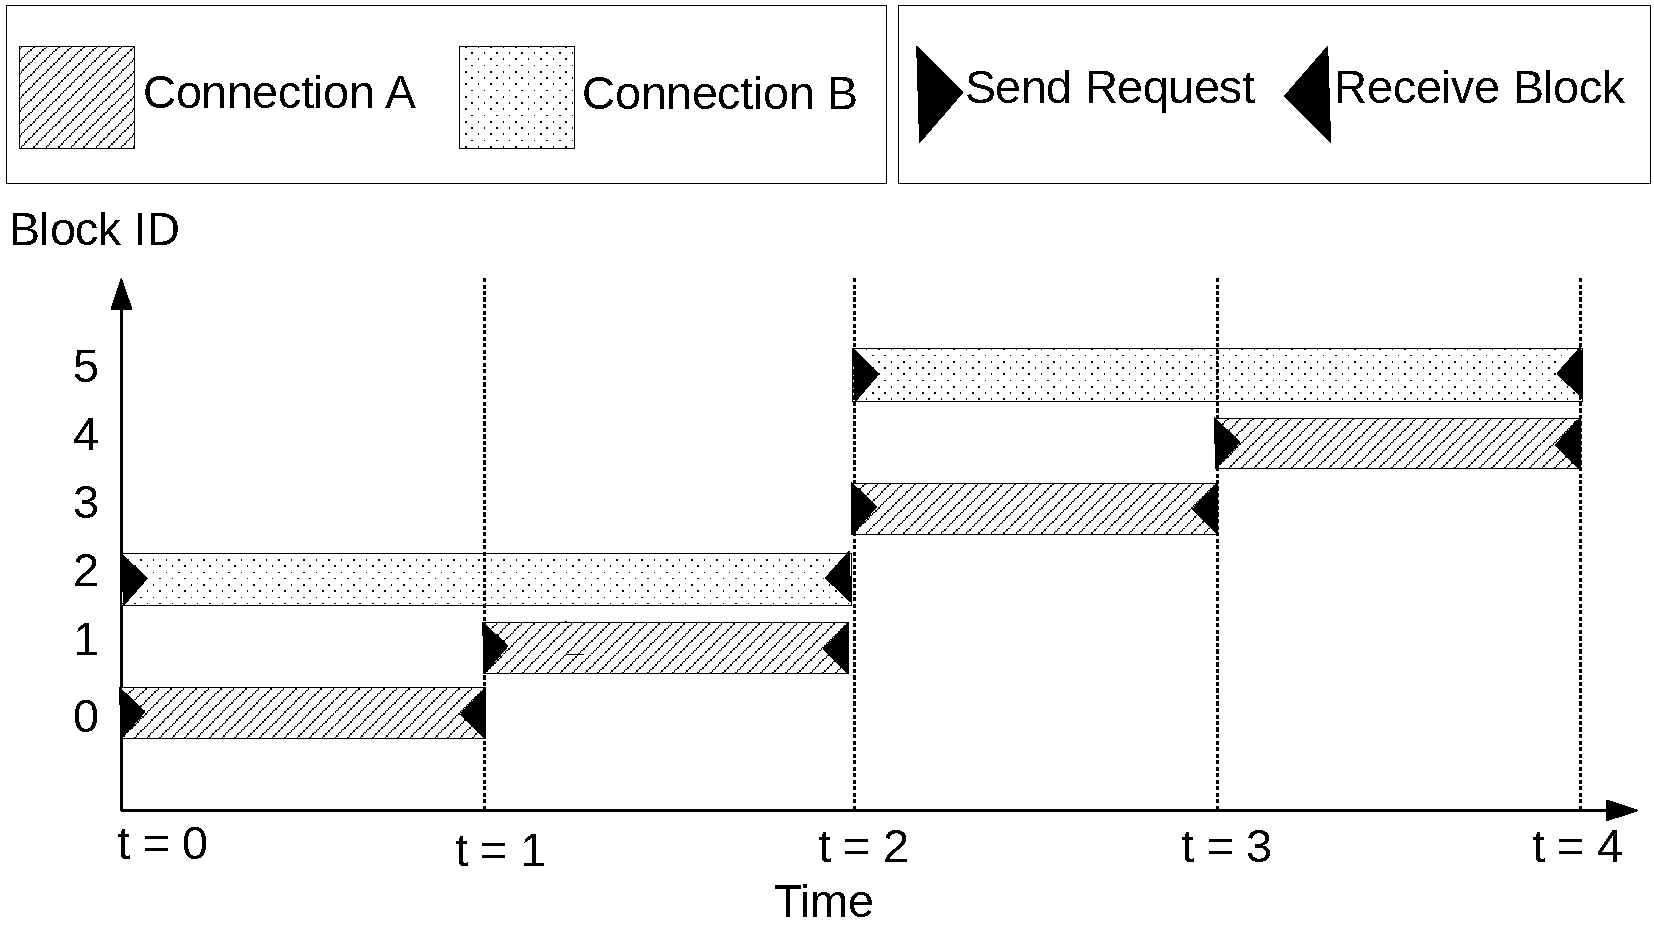
\includegraphics[width=7.6cm]{figure/delay.pdf}
	\vspace{-4mm}
	\caption{遅延要求の模式図}
	\label{delay}
\end{figure}
\vspace{-12mm}

\section{実験と評価}
\vspace{-3mm}
提案方式を実装したHTTPクライアントを用いてテストベッドと公開ネットワークで評価を行なった.
本稿では紙面の都合上,公開ネットワークでの結果のみを掲載する.
公開ネットワークでの実験には利用のしやすさからUbuntuのイメージファイルのパブリックミラーを利用した.
サーバは国内2つ,国外7つの合計9つ利用した.
事前に調査したミラーサーバにおける帯域性能の調査より,国内のサーバと国外のサーバの帯域性能差はおよそ6から46倍程度であることがわかっている.
各方式10回ずつファイル取得を行い,平均値を比較する.
また,取得するファイルは,映像と音声合わせてビットレートが40Mbpsで長さが150秒の動画の取得を仮定し,754MByteのイメージファイルを選択した.
評価対象は,先行研究で提案されている重複再要求のみを実装したもの(NORMAL)と,重複再要求に加えて提案方式である差分計測を用いた遅延要求方式を実装したもの(DIFF)の2種類である.
評価項目は,初期バッファリング時間,バッファ内の非有効ブロックの数,平均遅延時間である.
初期バッファリング時間とはグッドプット相当の再生レートの動画を,
途中停止することなく再生するために必要な再生開始時の待ち時間である.
この時間が短くなれば再生開始時の待ち時間が短縮される.
非有効ブロック数は取得したにもかかわらず,再生が不可能なブロックである.
平均遅延時間は各ブロックが理想的な到着時刻からの正の遅延時間の平均値である.
これらの値が小さいほど,複数のTCP接続を確立し得られた合計帯域をより有効に利用できているといえる.
実験結果を表\ref{hyoka}に示す.
値は平均値,標準偏差の組で表す.
10回試行の各ブロックIDにおける非有効ブロック数と平均遅延時間をプロットしたものを図\ref{testnsb},\ref{testadt}に示す.
\vspace{-8mm}
\begin{table}[htb]
	\begin{center}
		\caption{実験結果}
		\vspace{-0.5mm}
		\label{hyoka}
		\scalebox{0.65}{
		\begin{tabular}{|c|c|c|c|} \hline
			方式 & 初期バッファリング時間[s] & 平均非有効ブロック数 & 平均遅延時間[s]\\ \hline \hline
			NORMAL & 6.203, 0.717 & 6.435, 0.657 & 1.550, 0.322 \\ \hline
			DIFF & 3.130, 0.592 & 3.730, 0.390 & 0.866, 0.261 \\ \hline
		\end{tabular}
		}
	\end{center}
\end{table}
\vspace{-11.25mm}
\begin{figure}[h]
	\centering
	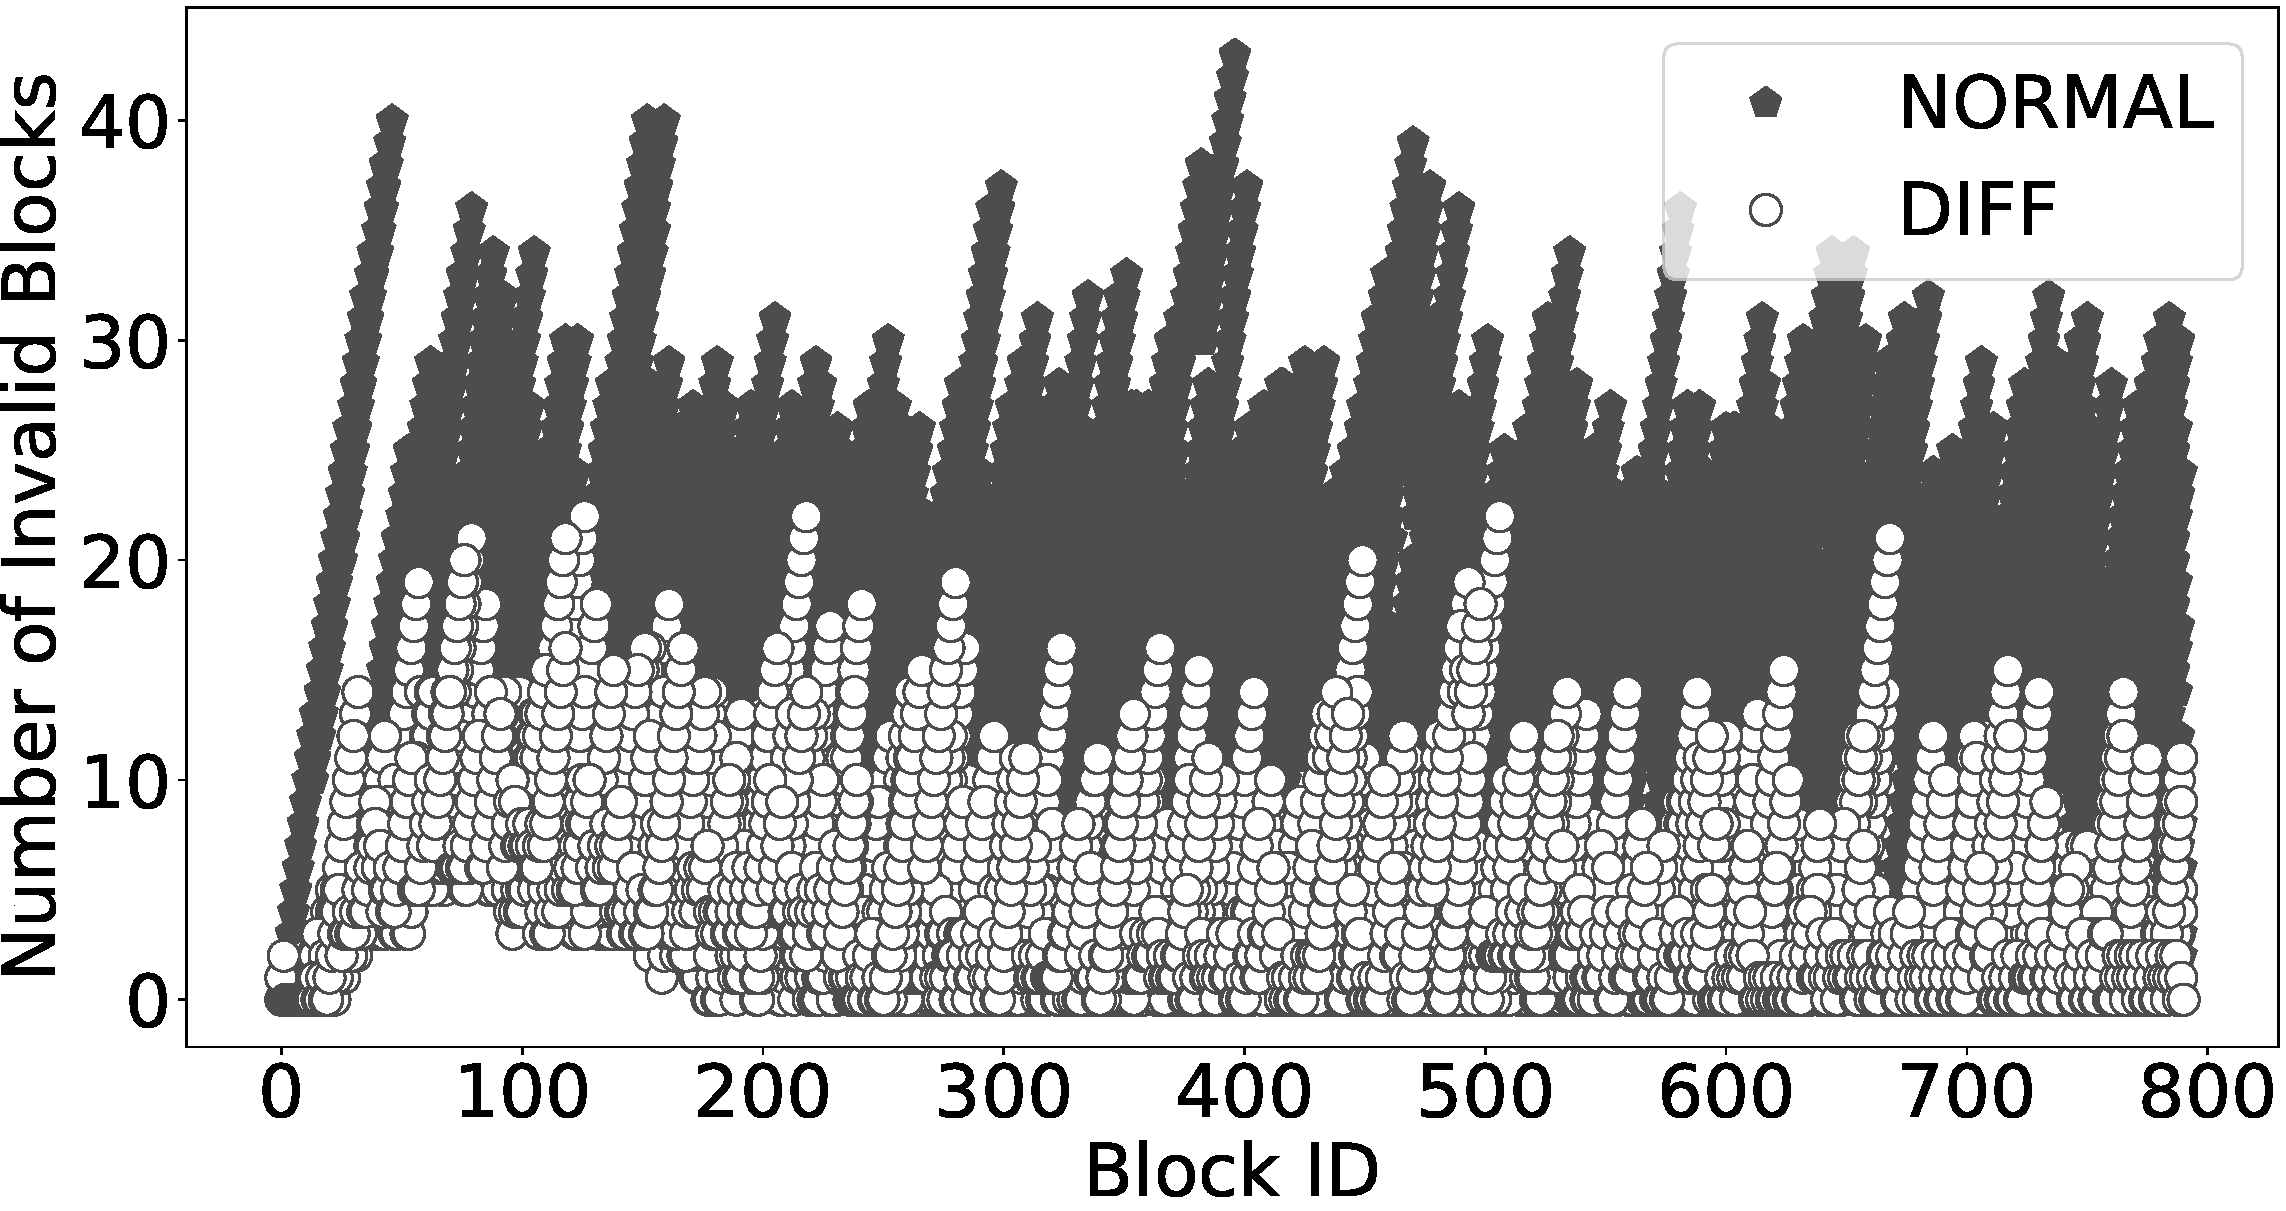
\includegraphics[width=8cm]{figure/testNSB.pdf}
	\vspace{-4.5mm}
	\caption{非有効ブロック数}
	\label{testnsb}
\end{figure}
\vspace{-4.5mm}

\vspace{-4mm}
\begin{figure}[h]
	\centering
	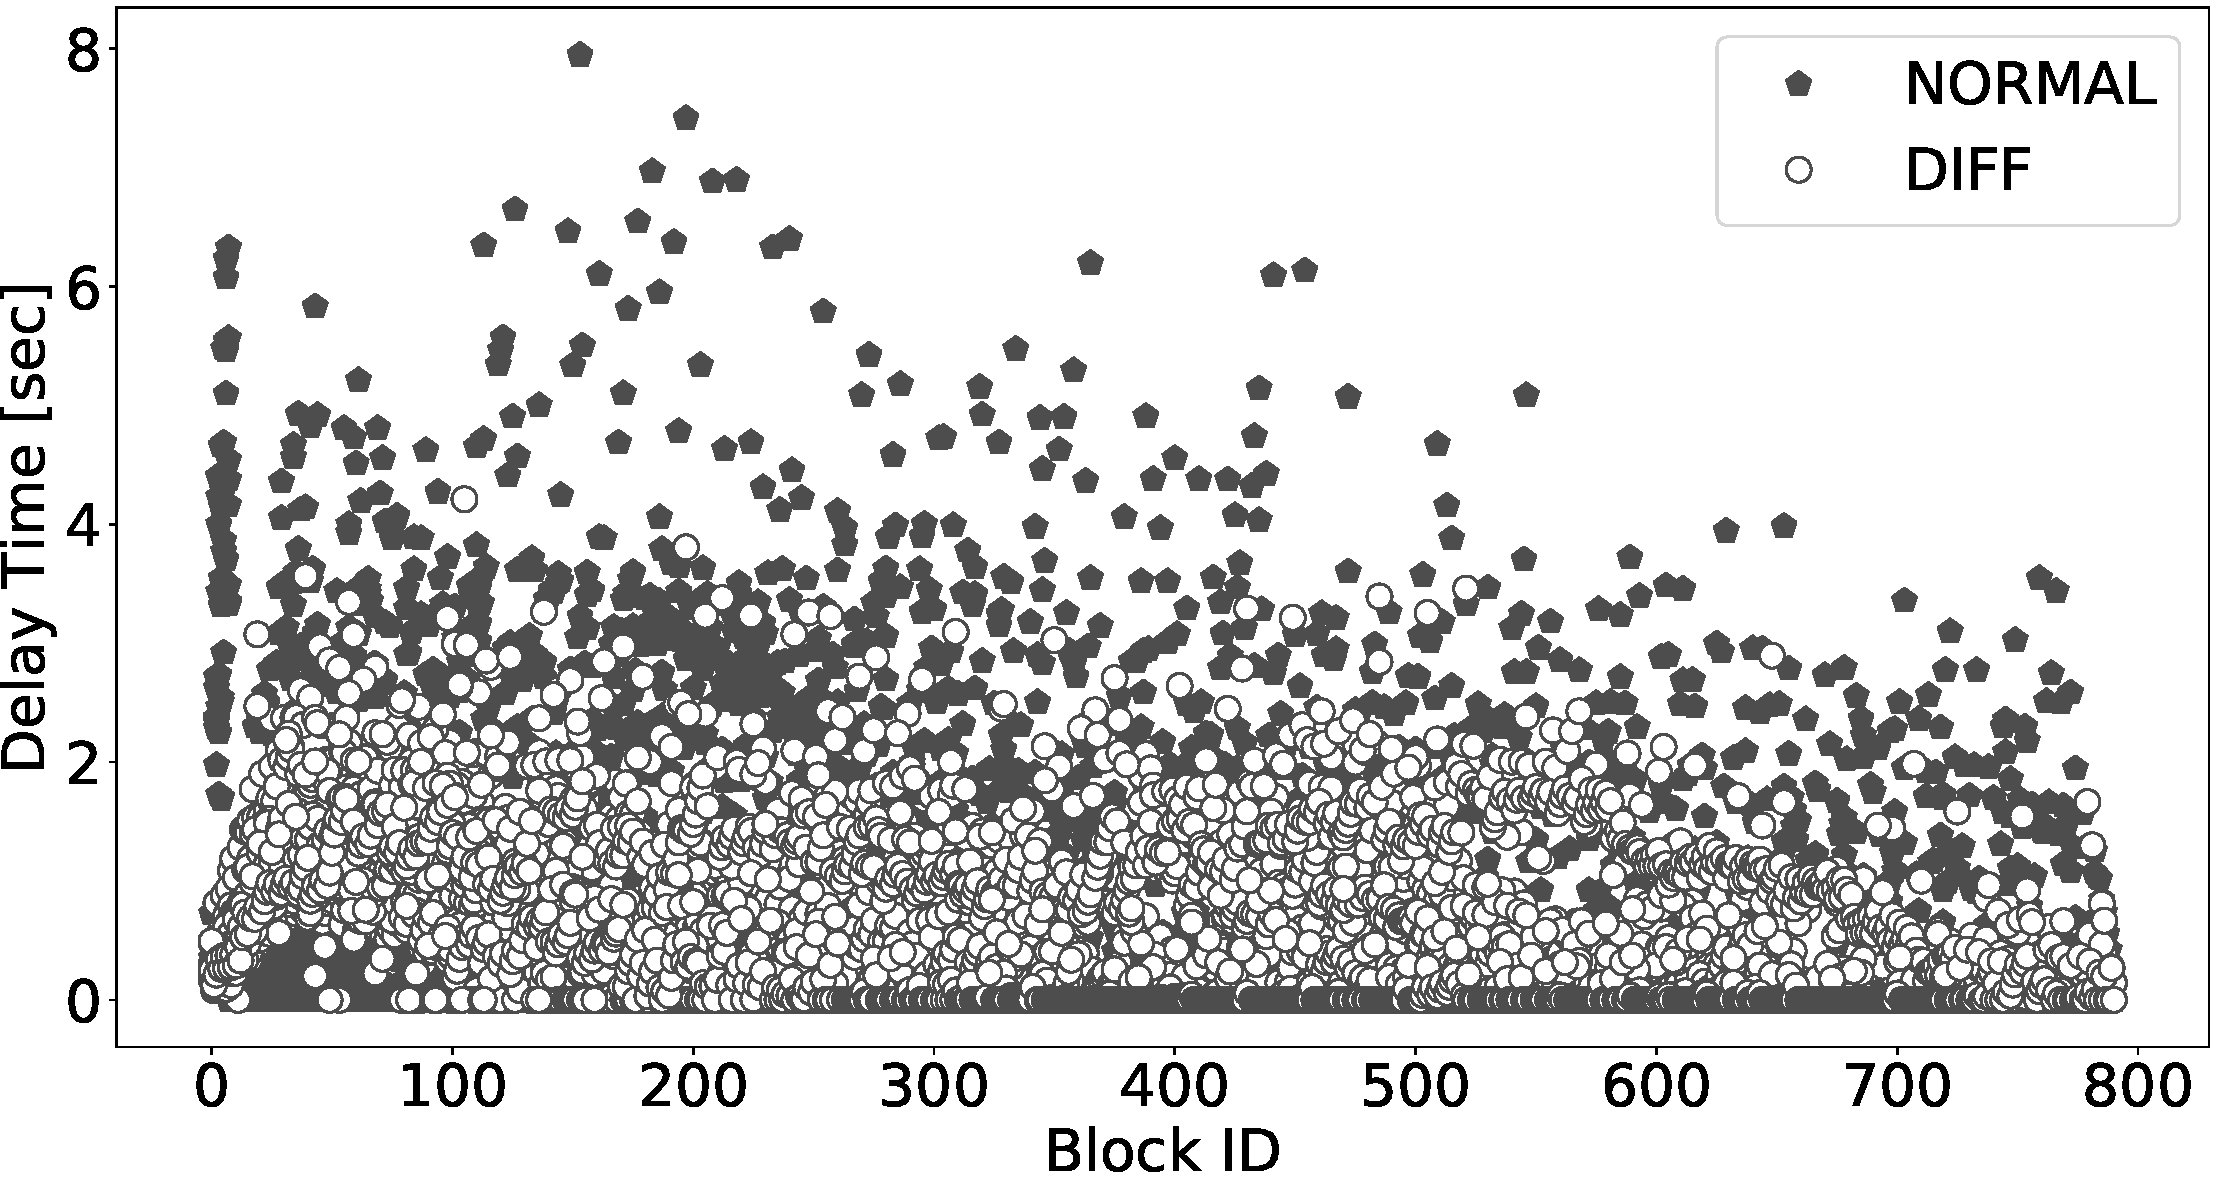
\includegraphics[width=8cm]{figure/testADT.pdf}
	\vspace{-4.5mm}
	\caption{平均遅延時間}
	\label{testadt}
\end{figure}
\vspace{-4.5mm}

\hspace{-3.5mm}表\ref{hyoka}より,公開ネットワークでの評価おいて提案方式は重複再要求のみの場合と比較して,
約50\%の初期バッファリング時間の短縮,約30\%の非有効ブロック数の削減,約30\%の平均遅延時間の短縮できたことが確認できる.
\vspace{-8mm}
\section{まとめ}
\vspace{-3mm}
複数のサーバから同一のファイルを並列に分割ダウンロードする際の順序逆転の発生を抑制する要求方式を提案し,
実装したHTTPクライアントをテストベッドと公開ネットワークで評価し優位性を確認した.
今後の課題としては,プロキシとして組み込んだシステムでの実際の動画の視聴体験まで含めた評価などが考えられる.
\vspace{-7.75mm}
%%%%%%%%%%%%%%%%%%%%%%%%%%%%%%%%%%%%%%%%%%%%%%%%%%%%%%%%%%%%%%%%%%%%%%%%%%
% 参考文献
%%%%%%%%%%%%%%%%%%%%%%%%%%%%%%%%%%%%%%%%%%%%%%%%%%%%%%%%%%%%%%%%%%%%%%%%%%
\fontsize{6pt}{0pt}\selectfont{
\begin{thebibliography}{9}
\vspace{-3mm}
\bibitem{mhttp}
Juhoon Kim, Yung-Chih Chen, Ramin Khalili, Don Towsley, Anja Feldmann,
"Multi-source Multipath HTTP (mHTTP): A Proposal,"
ACM SIGMETRICS Performance Evaluation Review, vol.42, no.1, pp.583-584, 2014.
\vspace{-2.75mm}
\bibitem{proxy}
Junichi Funasaka, Atsushi Kawano, and Kenji Ishida: Adaptive Parallel Downloading Method for Proxy Systems, IEICE Trans., Vol.E90-B, no.4, pp.720-727, 2007.
\end{thebibliography}}

\end{document}
